\section{Implementierung}
In dem folgenden Abschnitt wird gezeigt, wie man technisch die Authentifizierung und Autorisierung umsetzt, ein API Gateway mit Hilfe von Ocelot verwendet, eine RabbitMQ zur Verfügung stellt und die unterschiedlichen Services miteinander in einem Netzwerk verknüpft und deployed.  

\subsection{Implementieren der Authentifizierung und Autorisierung}
Ein zentraler Teil bei Microservices ist die Authentifizierung sowie die Autorisierung. Es wurde sich für eine Identity Server mit OAuth2 entschieden. Die MySQL-Datenstruktur ergibt sich aus dem Datenmodell:

\begin{verbatim}
public class User
{
    [Required] public int Id { set; get; }
    public string Name { set; get; }
    public string Password { set; get; }
    public bool Active { set; get; }
    public string Role { set; get; }
}
\end{verbatim}

Als eindeutiger Identifier ist eine `Id` notwendig. Zusätzlich besitzt jeder User einen Namen, ein Passwort, ist im Standardfall aktiviert und es wird zwischen zwei Rollen unterschieden: `customer` und  `admin`. Wie zu erwarten hat die `admin`-Rolle mehr Berechtigung als ein `customer`. \\

Um den Identity Server einzurichten, müssen sogenannte NuGet-Pakete heruntergeladen werden. NuGet ist ein System, mit welchem Softwarebibliotheken bereitgestellt werden können. Diese Verweise werden zur Projektdatei hinzugefügt.

\begin{verbatim}
<PackageReference Include="IdentityServer4" Version="2.3.0" />
<PackageReference Include="IdentityServer4.AccessTokenValidation" Version="2.7.0" />
\end{verbatim}

In der `Startup.cs`, welche standardmäßig bei C\# .NET Projekten vorhanden ist, werden grundsätzlich Serverkonfigurationen initialisiert. Dies muss für den Identity Server ebenfalls getan werden.

\begin{verbatim}
(1)
var builder = services.AddIdentityServer()
.AddInMemoryIdentityResources(Config.GetIdentityResources()) 
.AddInMemoryApiResources(Config.GetApis())
.AddInMemoryClients(Config.GetClients())
.AddProfileService<ProfileService>();

services.AddTransient<IResourceOwnerPasswordValidator, ResourceOwnerPasswordValidator>();
services.AddTransient<IProfileService, ProfileService>();
	
	(2)
	services.AddAuthentication("Bearer")
	.AddJwtBearer("Bearer", options =>
{
   options.Authority = "http://identity_server_service";
   [...]
   options.Audience = "srapi";
});
\end{verbatim}  

Wie man feststellen kann, sind diese Konfigurationen schon recht umfangreich, obwohl es sich in dieser Version schon um eine sehr leichtgewichtige Implementierung von OAuth2 handelt. In (1) wird der Identity Server zum Projekt hinzugefügt. Zusätzlich wird auf den `ProfileService` sowie den `ResourceOwnerPasswordValidator` verwiesen, welche anschließend initialisiert werden müssen. In (2) wird noch die `Authority` und die `Audience` gesetzt. Die `Authority` garantiert zusätzlich, dass das Token nicht von einem anderen Identity Server ausgestellt wird. Die `Audience` gibt noch einmal an, dass das ausgestellte Token nur Zugriff auf eine entsprechende `srapi` (Stirnraten-API) Ressource hat. 

\begin{verbatim}
new ApiResource("srapi", "Stirnraten API")
{
    ApiSecrets = new List<Secret>()
    {
    new Secret(CustomClientSecret.Sha256())
    }
}
\end{verbatim}

Zusätzlich müssen noch die beiden in den Grundlagen erwähnten Flows (`ClientCredentials` und `ResourceOwnerPassword`) implementiert werden. 

\begin{verbatim}{
[...]
new Client
{
    ClientId = CustomClientId,
    AllowedGrantTypes = GrantTypes.ClientCredentials,
    ClientSecrets =
    {
    new Secret(CustomClientSecret.Sha256())
    },
    AllowedScopes =
    {
    "srapi"
    }
},

new Client
{
    ClientId = "sr.client",
    AllowedGrantTypes = GrantTypes.ResourceOwnerPassword,
    ClientSecrets =
    {
    new Secret("secret".Sha256())
    },
    AllowedScopes =
    {
    "srapi"
    }
}

\end{verbatim}

Durch diese Flows ist garantiert, dass die API grundsätzlich geschützt ist, d.h. dass nur die Stirnraten Apps auf basale Funktionen der API zugreifen dürfen.  Wenn Benutzer in den Apps Benutzerdaten hinterlegt haben, erhalten diese logischerweise noch weitere Zugriffsrechte. Ein Konto mit der Rolle `admin` hat dementsprechend noch mehr Rechte. Dies wird im Abschnitt \ref{sec:umsetzung_api_gateway} deutlich. \\

Wenn eine Anfrage mit Benutzernamen und Passwort gestellt wird, ruft der Identity Server in seinem Abarbeitungszyklus folgende Methode ab: 

\begin{verbatim}
public async Task ValidateAsync(ResourceOwnerPasswordValidationContext context)
		{
		(1)
		var user = await _unitOfWork.UserRepository.
           GetUserByNameAndPasswordAsync(context.UserName, context.Password);
		
		(2)
		if (user == null)
		{
		context.Result = new GrantValidationResult(
		TokenRequestErrors.InvalidGrant,
		"invalid custom credential");
		return;
		}
		
		if (!user.Active)
		{
		context.Result = new GrantValidationResult(
		TokenRequestErrors.InvalidClient,
		"User was deactivated by admin");
		return;
		}
		
		(3)
		context.Result = new GrantValidationResult(
		subject: user.Id.ToString(),
		authenticationMethod: "custom",
		claims: GetUserClaims(user)); //get user claims
		}
\end{verbatim}

In (1) wird ein Benutzer gesucht, welcher mit dem übergebenen Namen und Passwort übereinstimmt. In (2) wird dieser validiert und in (3) das Token anhand der `Claims` generiert. `Claims` sind vereinfacht ausgedrückt, zusätzlich Informationen, welche man in dem Token übergeben möchte. 

\begin{verbatim}
return new[]
{
new Claim("user_id", user.Id.ToString() ?? ""),
new Claim(JwtClaimTypes.Name, user.Name),
new Claim(JwtClaimTypes.Role, user.Role)
};
\end{verbatim}

In der umgesetzten API wird eine `user\_id`, der `Name` sowie die `Role` übergeben. Alles wird ggf. von anderen Microservices benötigt, um eine entsprechende Autorisierung zu gewährleisten.\\

Abbildung \ref{fig:client_credentials_flow} und \ref{fig:password_flow} zeigen wie mit dem Programm Postman über eine POST Abfrage die entsprechenden Token ausgestellt werden können.\\

\begin{figure}[ht]
	\centering
	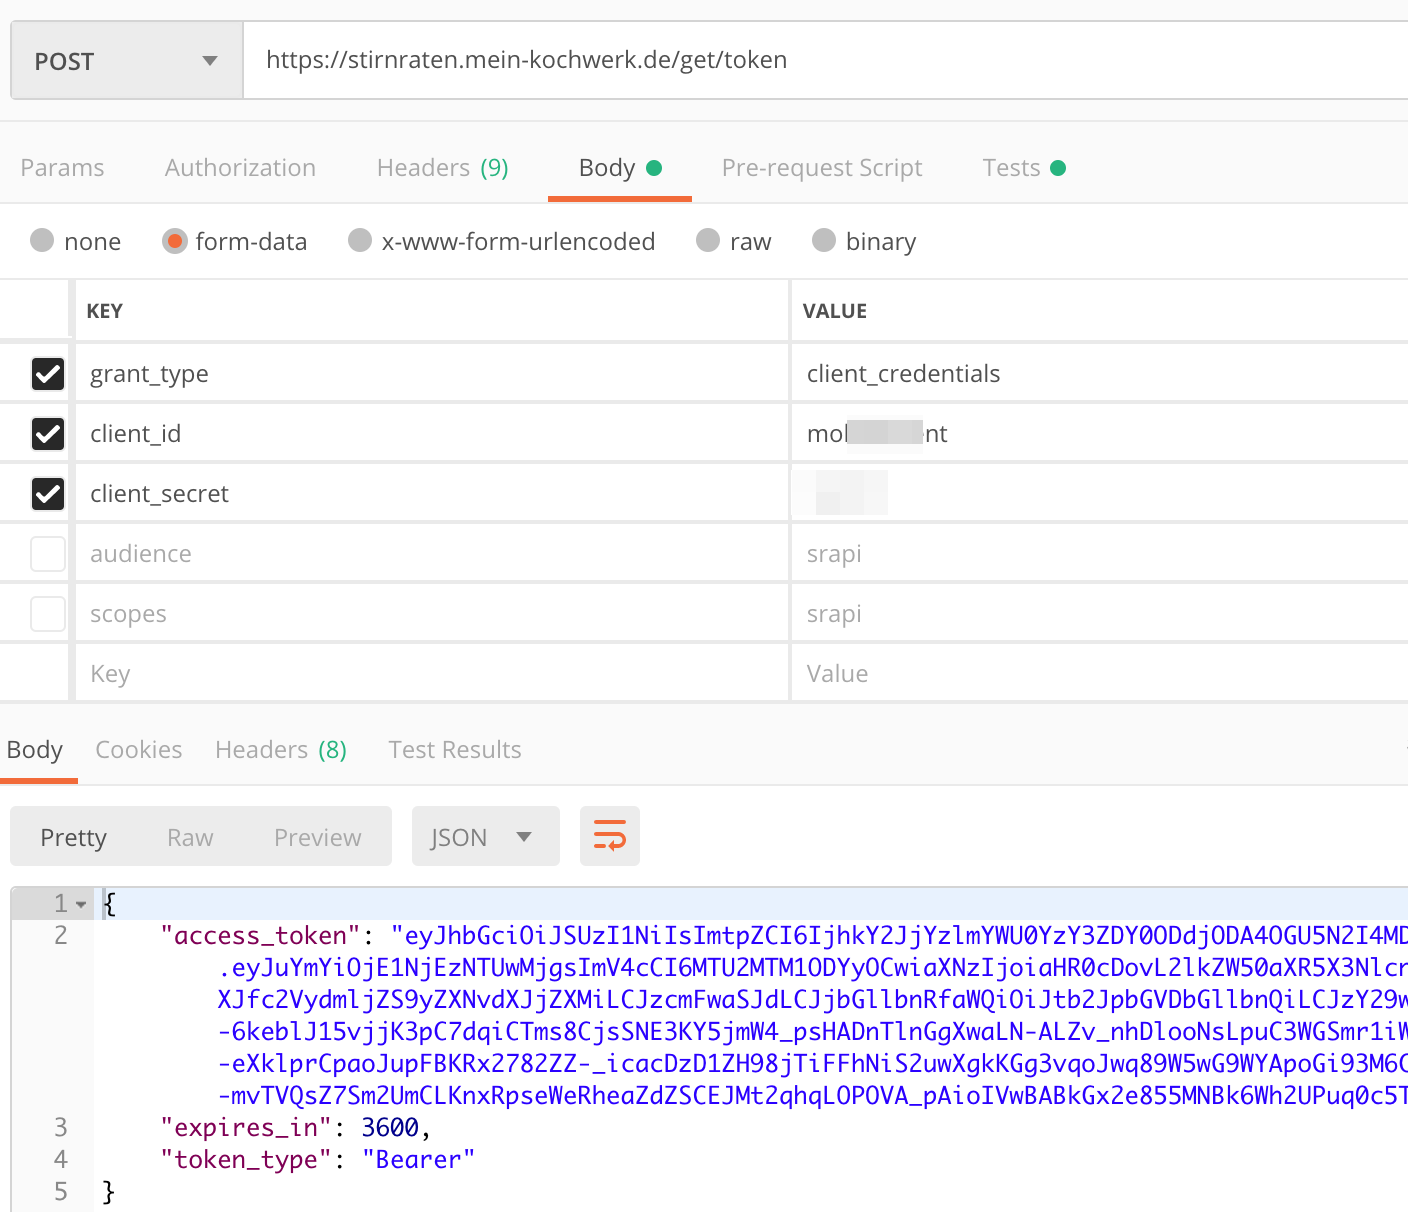
\includegraphics[width=0.6\textwidth]{client_credentials_flow}
	\caption[Über Postman gesendeter Client Credential Flow] {Über Postman gesendeter Client Credential Flow. Mit Hilfe dieses Tokens erhält man für 3600 Sekunden (eine Stunde) beschränkten Zugang zur API, um  z.B. Kategorien abzurufen, neue Wörter einzusenden oder ein Benutzerkonto anzulegen.}
	\label{fig:client_credentials_flow}
\end{figure} 

\begin{figure}[!ht]
	\centering
	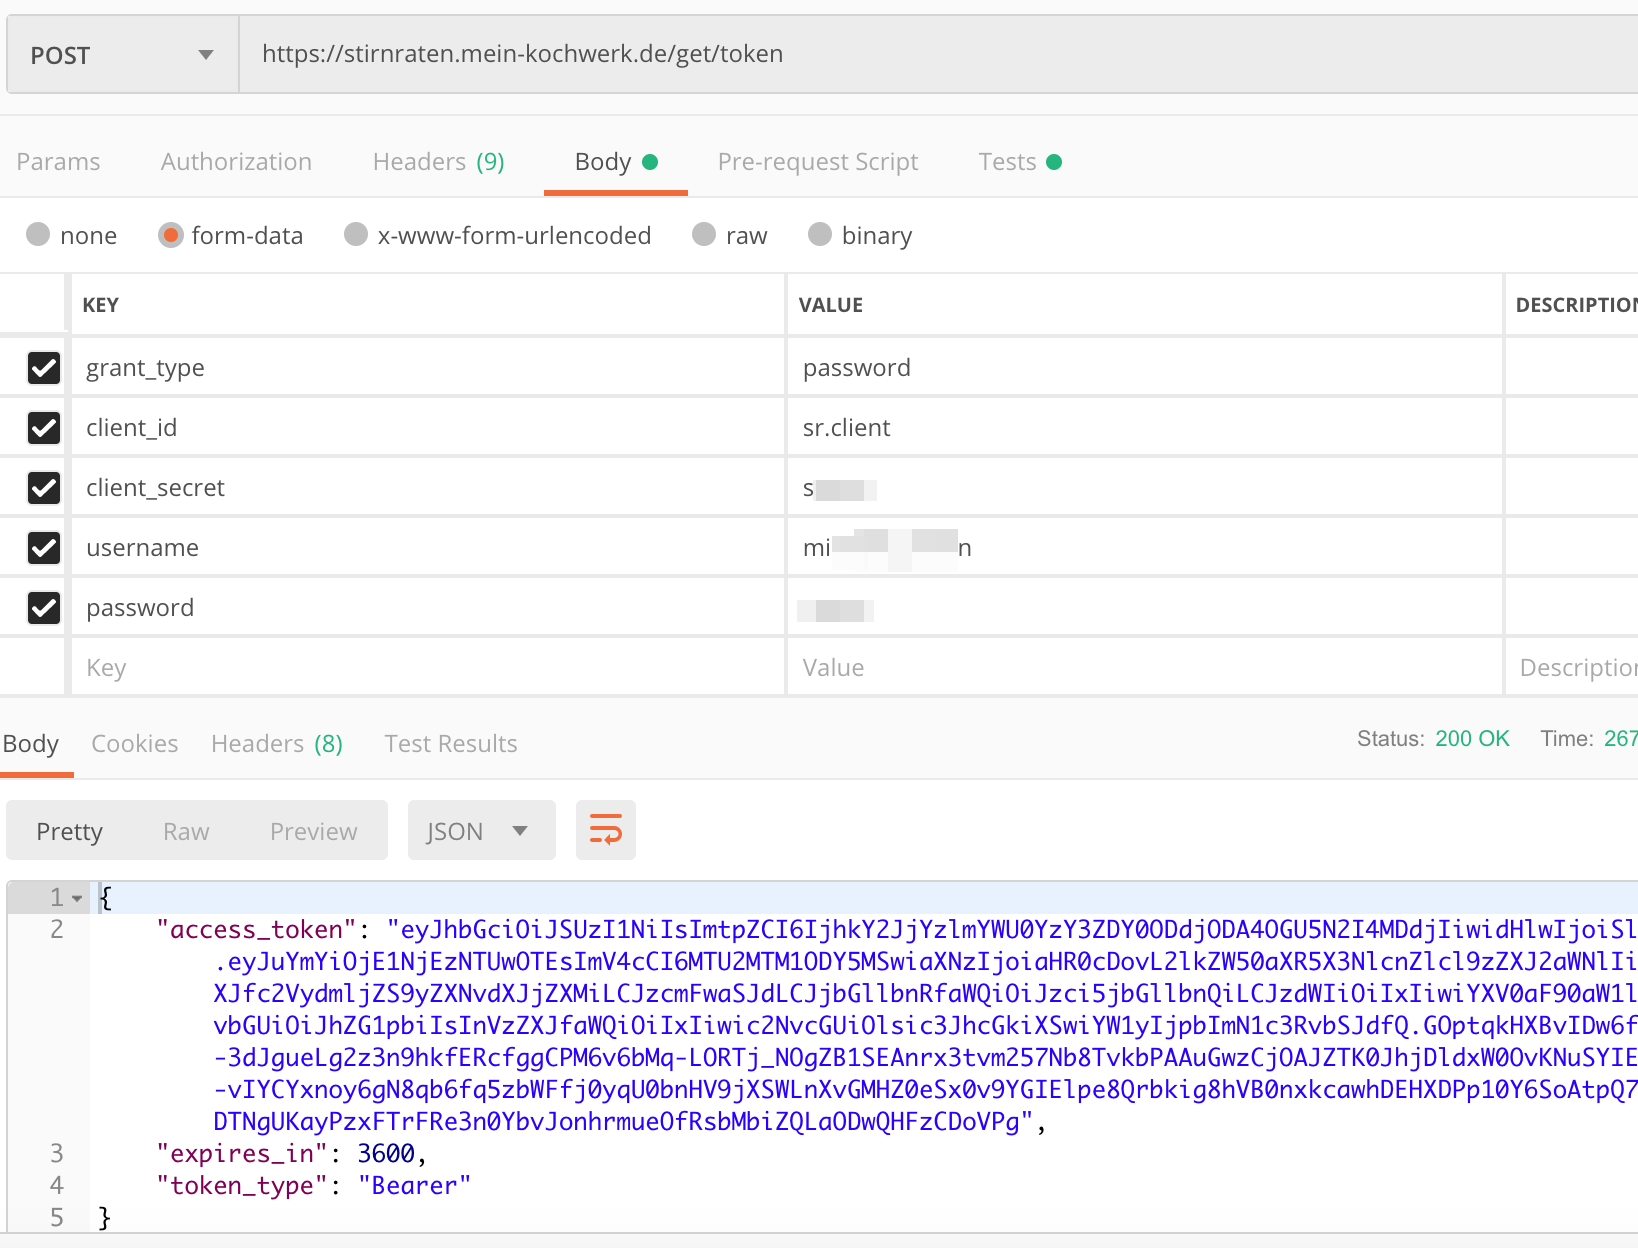
\includegraphics[width=0.6\textwidth]{password_flow}
	\caption[Über Postman gesendeter Password Flow] {Über Postman gesendeter Password Flow. Er ist ebenfalls 3600 Sekunden lang gültig und hat mehr Berechtigung, wie z.B. das Speichern eines Benutzerprofils.}
	\label{fig:password_flow}
\end{figure} \\

Enkodiert sieht so ein ausgestellter Benutzer-Token wie folgt aus: \\

\begin{verbatim}
		[...]
		"iss": "http://identity_server_service",
		"aud": [
		"http://identity_server_service/resources",
		"srapi"
		],
		"client_id": "sr.client",
		[...]
		"role": "admin",
		"user_id": "1",
		"scope": [
		"srapi"
		],
		"amr": [
		"custom"
		]
		[...]
\end{verbatim}  

Durch diese Informationen kann das API Gateway bereits eine Autorisierung vornehmen. Wie dies im Detail funktioniert, wird im Abschnitt \ref{sec:umsetzung_api_gateway} deutlich. 

\subsection{Implementierung des API Gateway mit Ocelot}\label{sec:umsetzung_api_gateway}

Ähnlich wie bei dem Identity Server müssen für Ocelot auch gewisse Bibliotheken über NuGet hinterlegt werden.

\begin{verbatim}
 <PackageReference Include="IdentityServer4.AccessTokenValidation" 
 Version="3.0.0-preview.2" />
<PackageReference Include="IdentityServer4" Version="2.4.0" />
<PackageReference Include="Ocelot" Version="11.0.2" />
<PackageReference Include="Microsoft.AspNetCore.Authentication.JwtBearer" />
\end{verbatim}

Durch diese Pakete wird zum einen Ocelot eingebunden, zum anderen wird der Authentifizierungsmechanismus zum Identity Server vereinfacht. Des Weiteren müssen Verbindungsdaten hinterlegt werden, die garantieren, dass das Gateway den Identity Server erreichen kann. Diese werden wieder in der `Startup.cs` hinterlegt.

\begin{verbatim}
(1)
var authenticationProviderKey = "NTT9N7MXLJN9";

(2)
void Options(IdentityServerAuthenticationOptions o)
{
   o.Authority = "http://identity_server_service";
   o.ApiName = "srapi";
   o.RequireHttpsMetadata = false;
   o.SupportedTokens = SupportedTokens.Both;
   o.ApiSecret = "xxxxxx";
}
services.AddAuthentication()
.AddIdentityServerAuthentication(authenticationProviderKey, Options);

[...]
(3)
await app.UseOcelot();
[...]
\end{verbatim}

In (1) muss ein sogenannter `Authentication Provider Key` gesetzt werden. Dies ist obligatorisch vorgegeben von Ocelot und notwendig, um weitergeleitete Requests eindeutig zuzuordnen. In (2) werden die Optionen für die Verbindung zum Identity Server definiert. Diese Konfigurationen müssen mit den Einstellungen aus dem zuvor erwähnten Identity Server übereinstimmen. In (3) wird noch einmal explizit ausgedrückt, dass Ocelot auch verwendet werden soll. \\

Um eingehende Request zu verarbeiten, verwendet Ocelot eine JSON, in der sogenannte ReRoutes (Weiterleitungen) hinterlegt werden. 

\begin{verbatim}
"ReRoutes": [
 {
 (1)
 "DownstreamPathTemplate": "/api/customers",
 (2)
 "DownstreamScheme": "http",
 "DownstreamHostAndPorts": [
    {
    (3)
    "Host": "customer_service",
    "Port": 80
    }
  ],
  (4)
  "UpstreamPathTemplate": "/api/stats",
  (5)
  "AuthenticationOptions": {
  "AuthenticationProviderKey": "NTT9N7MXLJN9",
  "AllowedScopes": [
    "srapi"
  ]
  },
  (6)
  "RouteClaimsRequirement": {
  "role": "admin"
  }
 },
[...]
]
\end{verbatim}

Diese dargestellte ReRoute zeigt bereits viele Vorteile von Ocelot. Durch (1) wird das `DownstreamPathTemplate` definiert. D.h. das Gateway präsentiert über das `UpstreamPathTemplate` (5) die öffentlichen Schnittstellen, welche man als Client anspricht. Dadurch lässt sich das Weiterleiten flexibel gestalten. Zusätzlich ist es nicht zwingend notwendig, dass wenn das `DownstreamPathTemplate` seine Route ändert, die Clienten davon betroffen sind, da das `UpstreamPathTemplate` gleichgeblieben ist. \\

Das `DownstreamScheme` (2) ist http, da die Microservices zu denen weiterleitet wird, sich nur in einem lokalen Netz befinden. Das hat den Vorteil, dass die Microservices nur über das Gateway zu erreichen sind. So kann garantiert werden, dass kein Dritter Zugriff auf die Services hat, ohne über das Gateway zu gehen. \\

In (3) wird definiert, an welchen Microservice weitergeleitet werden soll. In diesem Beispiel der `customer\_service`.\\

In (5) findet die Authentifizierung statt: Jeder Request, welcher eingeht, muss im Token als Scope die `srapi` enthalten. In diesem Beispiel wird bereits auch autorisiert. Denn es wird die Rolle `admin` erwartet (6). D.h. wenn ein Request kein gültiges Token oder die entsprechende Rolle hat, wird der Request abgelehnt. \\

Ocelot bietet zusätzlich an, Informationen aus dem Token direkt in den Request-Header zu parsen. Das kann sinnvoll sein, wenn der verarbeitende Service mit Daten aus dem Token arbeiten muss. Zum Beispiel darf ein Benutzer nur seine eigene Statistik sehen und verändern oder wenn ein neuer Benutzer angelegt wird, darf dieser nur die Rolle `admin` von einem anderen `admin` erhalten.  

\begin{verbatim}
[...]
(7)
"AddHeadersToRequest": {
 "claims_user_id": "Claims[user_id] > value > |",
 "claims_role": "Claims[role] > value > |"
},
(8)
"UpstreamHttpMethod": [
 "Get",
 "Delete",
 "Patch"
]
[...]
\end{verbatim}

Ebenfalls lassen sich die HTTP Methoden über die `UpstreamHttpMethod` einschränken (8). Dies bietet zusätzliche Sicherheit und Einschränkungen. \\

Zusammenfassend lässt sich sagen, dass Ocelot sehr mächtig über die JSON konfigurierbar ist. Ocelot bietet noch weitere Funktionen an, die allerdings nicht in der Stirnraten API verwendet worden sind.  

\subsection{Aufsetzen einer RabbitMQ}

Um wie geplant eine asynchrone Kommunikation zu erreichen, wird auf eine RabbitMQ zurückgegriffen. Diese läuft als eigenständiger Dienst auf dem Server. Um dies ohne viel Aufwand zu erreichen, wird die RabbitMQ als Container gestartet. Anschließend kann sich über eine Oberfläche mit der RabbitMQ verbunden werden. Die Oberfläche vereinfacht die Handhabung, ist allerdings nicht notwendig. Wie die Containerisierung im Detail verwendet wird, ist in dem Abschnitt 'Bauen und Hochladen der Microservices' nachzulesen.\\

Wenn die RabbitMQ gestartet ist, können die Services sich mit dieser verbinden. Dafür benötigen sie folgende Bibliotheken:

\begin{verbatim}
<PackageReference Include="MassTransit" Version="5.5.1" />
<PackageReference Include="MassTransit.Autofac" Version="5.5.1" />
<PackageReference Include="MassTransit.RabbitMQ" Version="5.5.1" />
\end{verbatim}

Es muss ein sogenannter 'Contract' erzeugt werden, dies ist im Prinzip die Nachricht, die übertragen werden soll. In diesem Fall werden die Daten (`UserId` und `Name`) beim Erzeugen eines neuen Benutzers erstellt und durch die RabbitMQ übertragen.

\begin{verbatim}
public class UserCreated
{
public string UserId { get; set; }
public string Name { get; set; }
}
\end{verbatim}

Anschließend muss die `Startup.cs` mit folgenden Informationen angereichert werden: 

\begin{verbatim}
private void ConfigureBus(ContainerBuilder builder)
 {
 builder.Register(context =>
 {
  return Bus.Factory.CreateUsingRabbitMq(config =>
  { 
   (1)
   var host = config.Host(new Uri("rabbitmq://" + _rabbitMqPath), h =>
   {
   (2)
   h.Username("xxxxx");  
   h.Password("xxxxx");
   });
  });
 }).As<IBus, IBusControl, IPublishEndpoint>().SingleInstance();
}
\end{verbatim}

Jeder Service, der mit der RabbitMQ verbunden sein möchte, benötigt diese Konfiguration. Über die URI wird dem Service mitgeteilt, über welche Adresse er sich mit der RabbitMQ verbinden kann. Anschließend werden Benutzernamen und Passwort benötigt (2). Anschließend muss die RabbitMQ gestartet werden, dies geschieht ebenfalls noch in der `Startup.cs`.

\begin{verbatim}
busControl.Start();
\end{verbatim}

Wenn ein neuer Benutzer erstellt wird, wird folgendes Kommando abgesetzt.

\begin{verbatim}
await _busControl.Publish(newUserCreated);
\end{verbatim}

Alle Services, die sich auf diese Nachricht abonniert haben, erhalten nun die Informationen. Dies impliziert das `IConsumer` Interface.  

\begin{verbatim}
public class UserCreatedConsumer : IConsumer<UserCreated>
{
 public Task Consume(ConsumeContext<UserCreated> context)
 {
 (1)
 var user = context.Message;
 return TaskUtil.Completed;
 }
}
\end{verbatim}

Bei (1) liegt der Benutzer vor, so dass der Service die Daten verarbeiten kann, wie er es benötigt. 

\subsection{Bauen und Hochladen der Microservices}

Die Architektur für den Livebetrieb hat sich ein wenig erweitert, da ein Proxy (siehe Abbildung \ref{fig:stirnraten_live} `nginx`) hinzugekommen ist. Diese Möglichkeit wird in der Regel von Hostingdiensten angeboten oder kann z.B. mittels Docker selbst erstellt werden. Es wird nur als eine Weiterleitung genutzt, hat aber z.B. den Vorteil, dass Nutzer von außen nicht sehen, welche Technologien oder Systeme für die Stirnraten API verwendet werden. Dies schützt vor möglichen Angreifern.

\begin{figure}[ht]
	\centering
	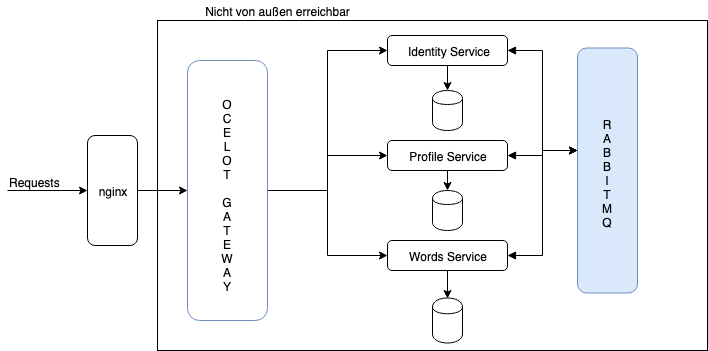
\includegraphics[width=0.7\textwidth]{stirnraten_live}
	\caption[Stirnraten Live Architektur] {Abbildung der Live-Architektur von der Stirnraten API}
	\label{fig:stirnraten_live}
\end{figure} 

Die Einstellung für den `nginx` beinhalten gerade einmal folgende Zeilen: 

\begin{verbatim}
<Location "/>
ProxyPass "http://127.0.0.1:6200/"
ProxyPassReverse "http://127.0.0.1:6200/"
</Location>
\end{verbatim}

Sobald ein Request eingeht, wird dieser auf an den Port 6200 weitergeleitet, wo der Ocelot Service läuft. Die Abbildung \ref{fig:stirnraten_live} zeigt insgesamt 8 Microservices. Das umfasst drei MySQL-Datenbanken, drei Services mit Geschäftslogik (Words, Customer, Identity Server), das Gateway und die RabbitMQ. Jeder dieser Services muss auf seinem eigenen Port laufen, um erreichbar zu sein und muss eigenständig deployed werden können.\\

Im Konzept wurde sich darauf festgelegt, dass die Microservices eigene Container sind. D.h. immer wenn ein Service gebaut wird, wird ein Docker-Image erzeugt. Das Bauen des Images wird über die Dockerfile beschrieben: 

\begin{verbatim}
(1)
FROM microsoft/dotnet:2.2-sdk
WORKDIR /app

(2)
# copy csproj and restore as distinct layers
COPY *.csproj ./
RUN dotnet restore
COPY . ./
RUN dotnet publish -c Release -o out
ENTRYPOINT ["dotnet", "out/GatewayService.dll"]
\end{verbatim}

In (1) wird beschrieben, welches .NET notwendig ist, in (2) wird in das Image eine ausführbare `dll` generiert. Dieses Image muss in eine Docker Registry. Für Unternehmen bietet es sich an, eine eigene Registry zu betreiben, der einfachhalber wegen, wurde für Stirnraten ein öffentlicher Dienst namens Dockerhub verwendet. Das Build-Script sieht exemplarisch wie folgt aus: 

\begin{verbatim}
docker build --tag kuzdu/stirnraten:gateway_service_live ../GatewayService
docker push kuzdu/stirnraten:gateway_service_live
\end{verbatim}

Über die Konsole mittels `build` wird ein Image erstellt und mit `gateway\_service\_live` getagged. Tags sind zum Identifizieren notwendig. Anschließend wird es nach Dockerhub übertragen. Hinweis: Um mit dem eigenen Dockerhub Account zu kommunizieren, muss man sich einmalig pro Gerät über die Konsole authentifizieren. \\

Wenn das Image nun in der Registry bereitliegt, muss der Live-Server es nur noch ausführen. Dieses Script sieht wie folgt aus:

\begin{verbatim}
#!/bin/bash
(1)
ssh root@mein-kochwerk.de << EOF 
(2)
docker stop stirnraten_gateway_service_live
docker rm stirnraten_gateway_service_live

(3)
docker run --restart unless-stopped --name stirnraten_gateway_service_live -p 127.0.0.1:6200:80 --network stirnraten -d kuzdu/stirnraten:gateway_service_live
exit
EOF #end of file
\end{verbatim}
Mittels `ssh` wird sich mit dem Server (hier mein-kochwerk.de heißend) verbunden (1). Es wird überprüft, ob bereits ein Microservice läuft, wenn ja, wird dieser gestoppt und anschließend entfernt (2). In (3) wird sich über `kuzdu/stirnraten:gateway\_service\_live` das entsprechende Image aus dem Dockerhub-Repository geladen und ausgeführt. Beim Ausführen vergeben wir einen Namen, lassen das Gateway auf dem Port 6200 laufen und teilen mit, dass die Anwendung sich neustarten soll, falls sie abstürzen sollte. Sehr wichtig ist auch der `network` Parameter. Dieser fasst die Microservices in einem Netzwerk zusammen. Dies bedeutet, dass die Services innerhalb dieses Netzwerk problemlos kommunzieren können. Falls auf dem Server noch andere Container laufen, die gar nicht zur Anwendung gehören, sehen diese Container sich nicht.\\

Um eine bessere Übersicht zu behalten, wurde auf dem Server ein Dienst namens `Portainer` installiert. Dieser bietet zur Docker-Konsole eine grafische Oberfläche. In der Abbildung \ref{fig:portainer} sieht man alle Stirnraten-Container. 

\begin{figure}[ht]
	\centering
	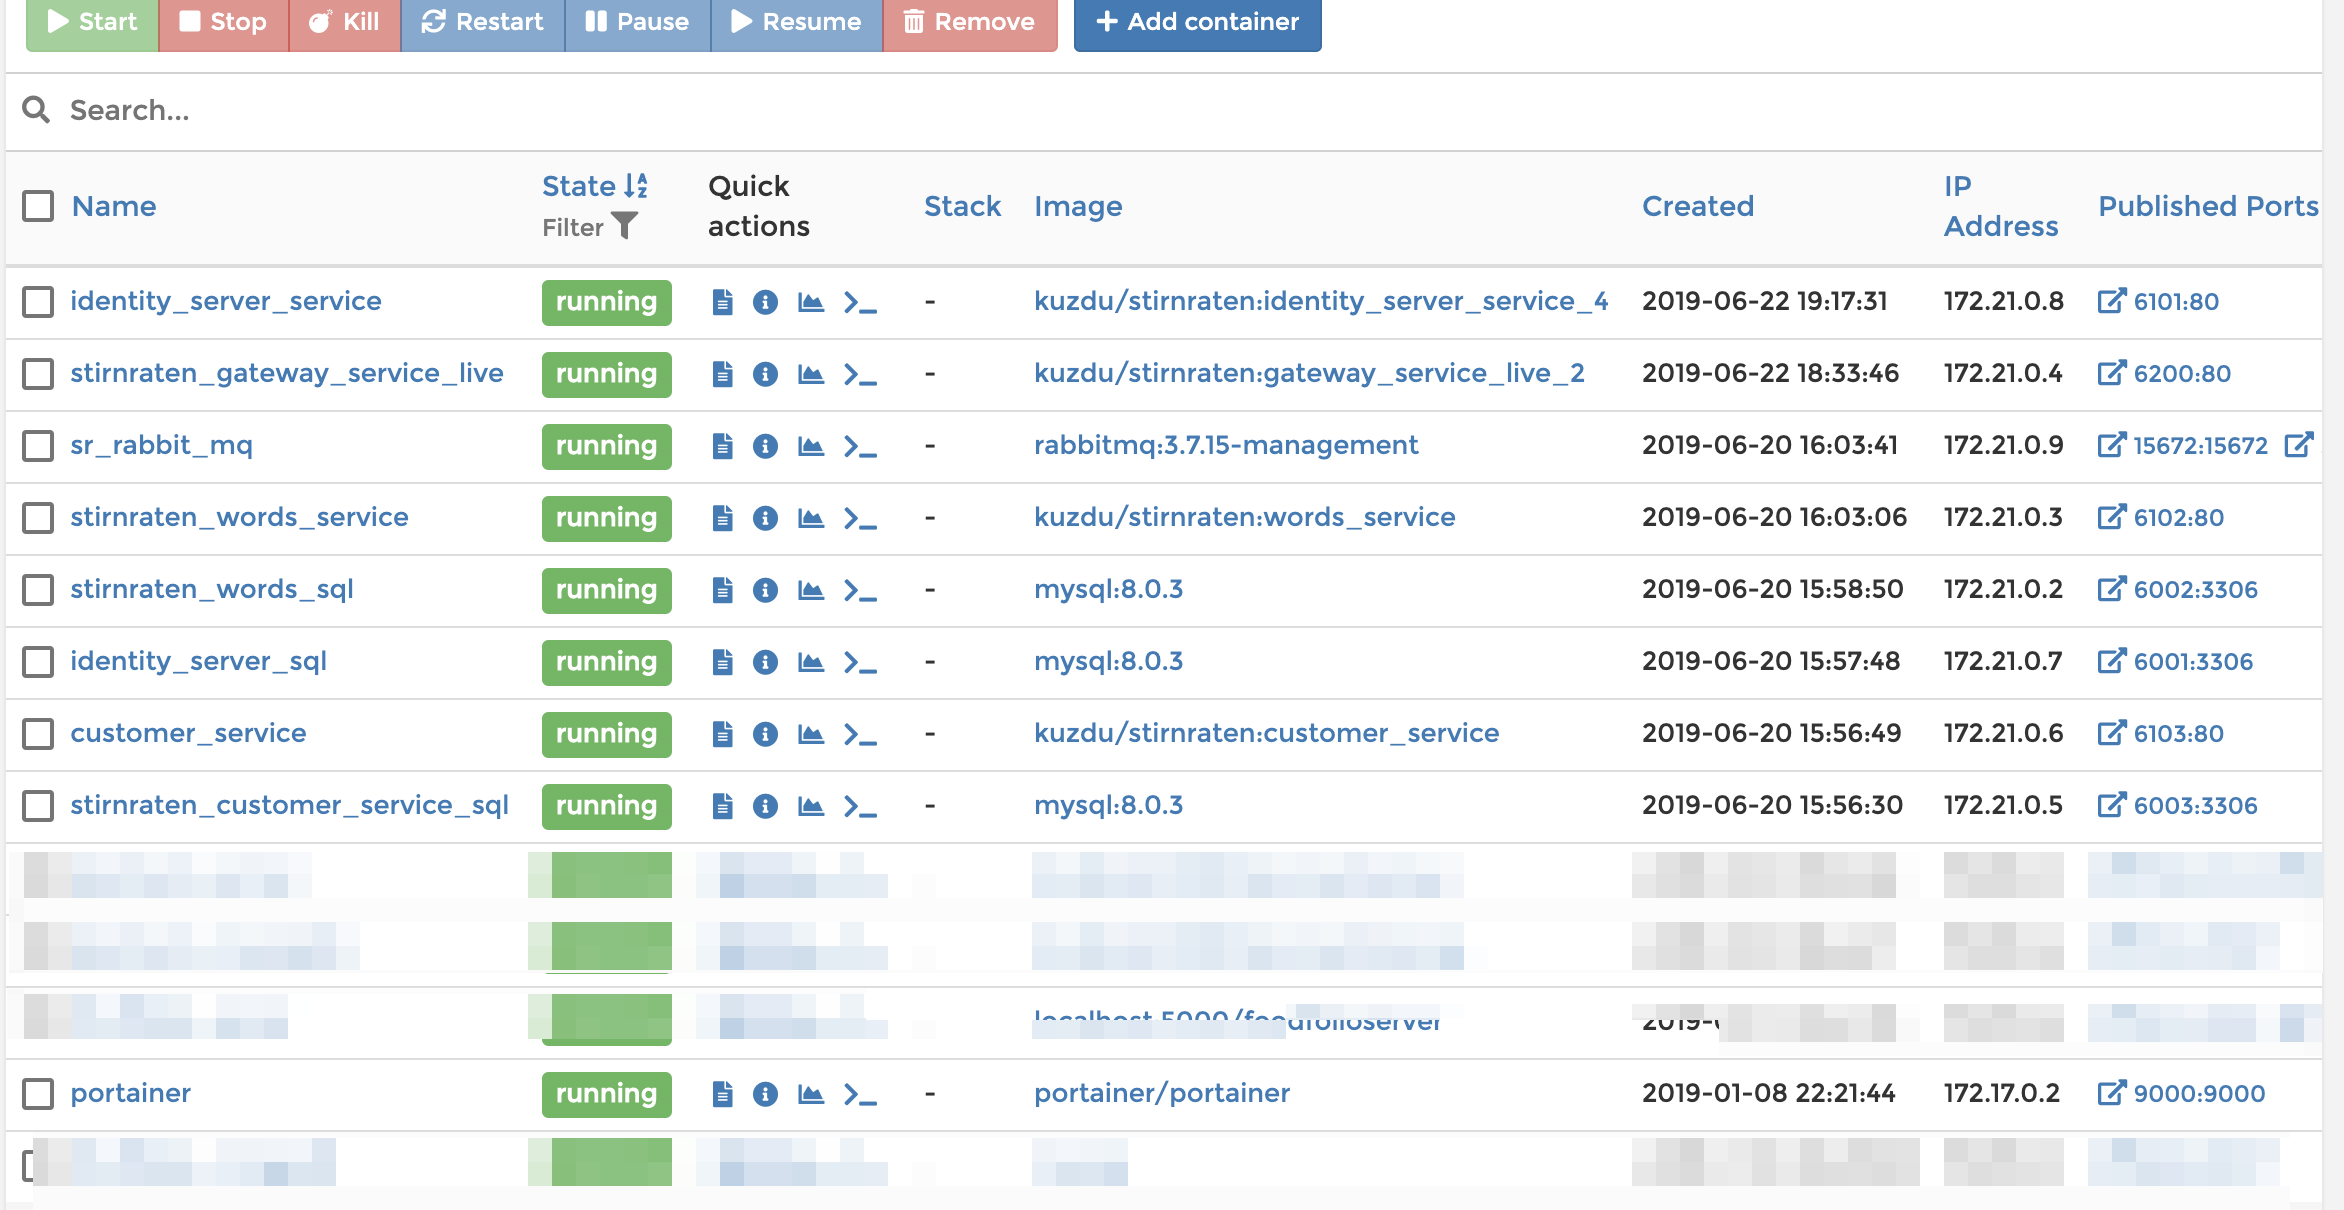
\includegraphics[width=0.8\textwidth]{portainer}
	\caption[Alle laufenden Microservices] {Alle laufenden Microservices}
	\label{fig:portainer}
\end{figure} 





